%Disposition
%Affektiv
%pyskotisk
%somatisk

\section{Affektive lidelser}\label{sec:affektivelidelser}
Dette afsnit er primært baseret på \citet{misc:affektivelidelser, misc:netpsykdepression, misc:netpsykmani, havemann2010grundbog}.

Affektive lidelser omfatter en række sygdomme hvor stemningslejet afviger fra det \textit{habituelle}. 
Stemningsleje er et begreb der dækker over humør og lyst.
Med habituelt stemningsleje menes en persons humør og adfærd når personen hverken befinder sig i depression eller mani-periode.
Et kendetegn ved sindslidelserne er at de forekommer periodisk.
For nogle vil dette være enkeltstående episoder, mens det for andre vil være tilbagevendende episoder.
Der er en stor dødelighed blandt patienter med affektive lidelser, grundet selvmord.

Stemningslejet kan afvige fra det habituelle på forskellig vis.
Her skelnes mellem mani og depression.
Ved depression er stemningslejet sænket, mens det ved mani er løftet.
Unipolare patienter lider af depression og oplever depressions-perioder.
Bipolare patienter derimod har haft minimum én mani-periode og eventuelt et antal depressions-perioder.

Der findes forskellige årsager til affektive lidelser. 
Disse inkluderer miljømæssige og arvemæssige forhold, især ved bipolare patienter.
Somatiske sygdomme såsom blodprop, hjerneblødning og Parkinsons kan også forårsage depression og mani.
Ud over dette kan diverse misbrug, samt bestemte former for medicinbrug, også forårsage mani og depression.

\subsection{Depression}
Risikoen for at udvikle en depression for kvinder er cirka 8\%, mens den for mænd er cirka 4\%.
Debutalderen for begge køn ligger almindeligvis mellem 40 og 50 år.
En ubehandlet sygdom varer typisk seks til tolv måneder.
Kroniske depressioner med op til flere års varighed er ikke ualmindelige især hos ældre.
Derudover har kun cirka 15\% af patienterne, en enkeltstående hændelse af depression, hvilket understreger at sygdommen ofte er tilbagevendende\citep{misc:affektivelidelser}.

\Citet{misc:netpsykdepression} klassificerer en depressiv enkeltepisode ud fra en række kriterier.
De følgende kriterier er taget direkte ud fra \citet{misc:netpsykdepression}.

\begin{mdframed}
\paragraph{Depression:}
For at opfylde kriterierne for at have en \textit{depressiv enkeltepisode} i lettere grad skal man:
\begin{itemize}
	\item Have haft depressionen i mere end 2 uger
	\item Ikke tidligere have haft en mani eller en let mani, en såkaldt hypomani
	\item Ikke have en fysisk lidelse som kan forklare symptomerne
\end{itemize}
Man skal have mindst 2 af følgende \textit{kernesymptomer}:
\begin{itemize}
	\item Man er i dårligt humør og er nedtrykt og trist
	\item Man har \textbf{nedsat} lyst til at foretage sig noget, og man har mere eller mindre mistet interessen for ting, man plejer at interessere sig for
	\item Man bliver hurtigt træt og har ikke så meget energi som man plejer
\end{itemize}
Desuden skal man have mindst 2 af følgende ledsagesymptomer:
\begin{itemize}
	\item Man har nedsat selvtillid eller selvværdsfølelse
	\item Man lider af skyldfølelse og bebrejder sig selv urimeligt
	\item Man har tanker om at det ville være bedre, hvis man var død, eller man tænker på at begå selvmord
	\item Man har svært ved at koncentrere sig eller oplever at man ikke kan tænke klart
	\item Man er enten urolig og hvileløs, eller også er ens bevægelser nærmest gået i stå
	\item Man sover enten mere eller mindre, end man plejer
	\item Man har mistet appetitten og har tabt sig, eller man er begyndt at trøstespise og har taget på
\end{itemize}
\end{mdframed}

\subsubsection{Grader af depression}
Man skelner mellem forskellige grader af depression.
Depression i lettere grad vil sige at man er i stand til at bibeholde sine sædvanlige aktiviteter, på trods af at man har nedsat stemningsleje.
Ved depression i moderat grad har man 4 ledsagesymptomer og som resultat af dette har man svært ved at forsætte med sine sædvanlige aktiviteter.
Har man en svær depression har man alle 3 kernesymptomer og 5 ledsagesymptomer.
Ved svær depression er man ikke i stand til at fortsætte med sine normale aktiviteter.

\subsubsection{Individuelle symptomer}
Det er vigtigt for patienter der lider af depression, at de er opmærksomme på hvad deres symptomer er.
Eksempler på dette kan være en overfladisk søvn, forøget bekymringer om bagateller eller forlænget søvn.
Disse symptomer vil for individet ofte følge med en depressions-periode.
Hvis disse symptomer opfanges, kan behandling af depressionen påbegyndes tidligere i forløbet og i bedste tilfælde kan svære episoder forhindres.
\subsubsection{Selvbehandling}
Man kan nedsætte risikoen for en depression hvis man har en sund livsstil.
Dette inkluderer at spise sund mad, dyrke motion og undgå at indtage rusmidler.
Desuden informerede kontaktpersonen Janne Vedel Rasmussen, se \cref{sec:moede-med-psykolog}, at til behandling af depression opfordres patienten til at foretage en mængde lystbetonede aktiviteter.
Lystbetonede aktiviteter værende ting, der plejer at få patienten til at føle sig glad, dette kunne for eksempel være at gå en tur i biografen eller tage ud at spise. 

\subsection{Mani}
Risikoen for at udvikle en mani, og derved en bipolar sygdom, er ca. 1-2\%, og er lige hyppig blandt mænd og kvinder.
Dog er det ofte at sygdommen er tilbagevendende, da der er en risiko på ca. 90\% for at få en ny episode på et senere tidspunkt.
Debutalderen for sygdommen er almindeligvis før 30-års alderen, og ved omkring halvdelen af patienterne forekommer sygdommen før man er 20 år.
Varigheden af sygdommen er i ubehandlede tilfælde typisk mellem to og otte måneder, men der findes her også kroniske tilfælde.

\citet{misc:netpsykmani} klassificerer en manisk enkeltepisode uden psykotiske symptomer som at man i mere end en uge skal opfylde følgende kriterier.
Kriterierne er taget fra \citet{misc:netpsykmani}.
\begin{mdframed}
\paragraph{Mani:}
For at opfylde kriterierne for at have \textit{en manisk enkeltepisode uden psykotiske symptomer} skal man i mere end en uge:
\begin{itemize}
	\item Have været opstemt, eksalteret og irritabel.
	\item Hvis man er opstemt eller eksalteret have mindst tre af følgende symptomer. Hvis man især er irritabel skal man op på mindst fire symptomer:
	\begin{itemize}
		\item Man er hyperaktiv, rastløs og urolig
		\item Man føler et indre pres for at tale uafbrudt
		\item Man har tankeflugt, hvor tankerne springer fra emne til emne
		\item Man har en hæmningsløs adfærd, hvor ens normale hæmninger er væk
		\item Man har nedsat behov for søvn
		\item Man har forhøjet selvfølelse, \textit{grandiositet}
		\item Man er usamlet eller bliver konstant distraheret
		\item Man handler hensynsløst og uansvarligt
		\item Man har større seksualdrift end normalt
	\end{itemize}
	\item Ikke have haft hallucinationer eller vrangforestillinger
	\item Symptomerne må ikke skyldes en fysisk sygdom
\end{itemize}
\end{mdframed}
Hvis man derimod har en \textit{manisk enkeltepisode med psykotiske symptomer} svarer den til symptomerne for en \textit{manisk enkeltepisode uden psykotiske symptomer}, men hvor man har haft hallucinationer eller vrangforestillinger. Dog ikke bizarre vrangforestillinger såsom ved skizofreni.

\subsubsection{Individuelle symptomer}
Det er individuelt hvilke symptomer de enkelte patienter har på en begyndende mani-periode.
Dog starter perioden ofte på samme måde som tidligere perioder.
Eksempelvis kan man være meget aktiv, rastløs, have mindre brug for søvn eller være ekstatisk.

Ligesom depression er det vigtigt at opdage episoderne i de begyndende stadier, da man på den måde ville kunne mindske eller helt undgå episoden.
Derudover kan en depression følge efter en mani-periode og man kan derfor også mindske risikoen for disse episoder \citep{misc:bipolarsundhed}.

\subsubsection{Selvbehandling}
Man skal undgå at drikke alkohol når man er i en mani-periode, da det kan forværre perioden \citep{misc:netpsykmani}.
Derudover beretter Janne Vedel Rasmusse (se \cref{sec:moede-med-psykolog}), at man også bør begrænse mængden af stimuli og generelt forsøge at tage det mere med ro.

\subsection{Unipolar lidelse}
En unipolar lidelse er kendetegnet ved folk, der har lidt af minimum én depressions-periode og ingen mani-perioder.
Hvis en person med unipolar lidelse har en mani-periode, bliver deres klassificering ændret til bipolar lidelse.

Ifølge \citet{misc:netpsykdepression} har omkring hver femte person, der får en depression, kun den ene periode og hver tiende får mere end ti.

\subsection{Bipolar lidelse}
Bipolar lidelse er kendetegnende ved minimum én mani episode og evt. depressions episoder.
I \cref{fig:stemningslejegrafeksempel} gives et eksempel på dette.
Her viser en graf et eksempel på en patients stemningsleje over tid.

\begin{figure}
	\centering
	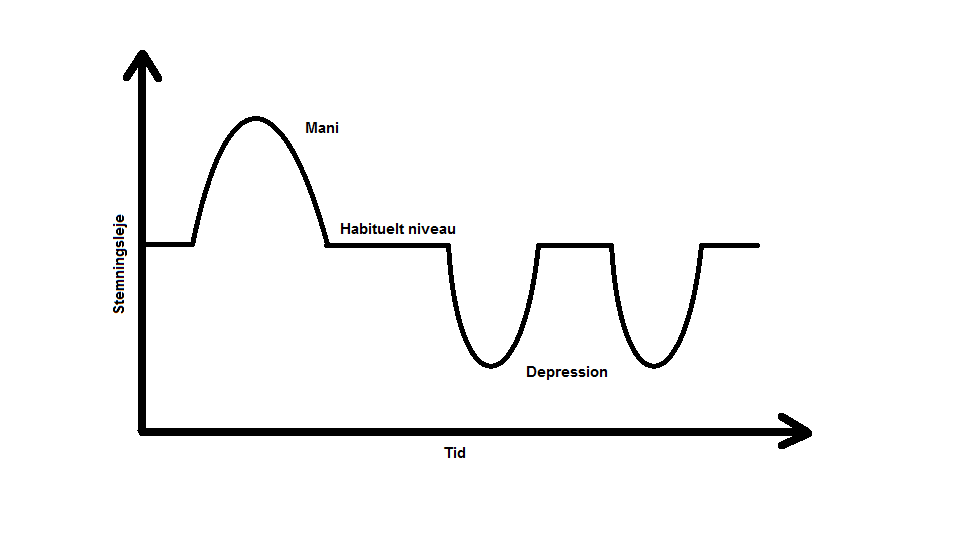
\includegraphics[scale=0.5]{affektivstemningsleje}
	\caption{Graf over stemningsleje for en patient med en mani og to depressionsperioder.}\label{fig:stemningslejegrafeksempel}
\end{figure}

Det oftest sete er en mani episode og flere depressions episoder, men andre scenarier kan også forekomme.
Det gælder således om at have patienten på det habituelle niveau og hurtigst muligt opdage når en patient afviger fra dette.